\contourlength{1.0pt}
\tikzset{>=latex} % for LaTeX arrow head

\colorlet{xcol}{blue!60!black}
\colorlet{myred}{red!80!black}
\colorlet{myblue}{blue!80!black}
\colorlet{mygreen}{green!40!black}
\colorlet{myorange}{orange!90!black}
\colorlet{mypurple}{red!50!blue!90!black!80}
\colorlet{mydarkred}{myred!80!black}
\colorlet{mydarkblue}{myblue!80!black}
\tikzstyle{xline}=[xcol,thick]
\tikzstyle{width}=[{Latex[length=5,width=3]}-{Latex[length=5,width=3]},thick]
\tikzset{
  traj/.style 2 args={xline,postaction={decorate},decoration={markings,
    mark=at position #1 with {\arrow{<}},
    mark=at position #2 with {\arrow{<}}}
  }
}
\def\tick#1#2{\draw[thick] (#1)++(#2:0.12) --++ (#2-180:0.24)}
\def\N{100} % number of samples

% CIRCLE on axis




% COS - damped


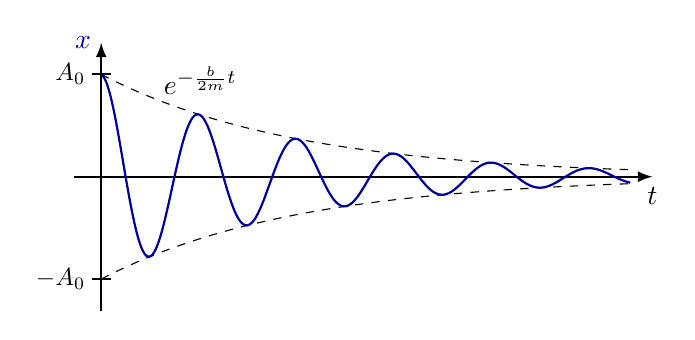
\begin{tikzpicture}
  \def\xmax{7.0} % max x axis
  \def\ymax{1.7}
  \def\A{1.3}
  \def\om{(5.3*360/(0.94*\xmax))}
  \def\t{1800/(0.94*\xmax)}
  \def\T{2.5}
  
  % AXIS
  \draw[->,thick] (0,-\ymax) -- (0,\ymax) node[left,xcol] {$x$};
  \draw[->,thick] (-0.2*\ymax,0) -- (\xmax,0) node[below] {$t$};
  \tick{0,\A}{0} node[left=-1,scale=0.9] {$A_0$};
  \tick{0,-\A}{0} node[left=-1,scale=0.9] {$-A_0$};
  
  % PLOT
  \draw[dashed,samples=\N,smooth,variable=\t,domain=0:0.96*\xmax]
    plot(\t,{\A*exp(-\t/\T)}) plot(\t,{-\A*exp(-\t/\T)});
  \draw[xline,samples=100+\N,smooth,variable=\t,domain=0:0.96*\xmax]
    plot(\t,{\A*exp(-\t/\T)*cos(\om*\t)});
  \node[above=4] at (0.18*\xmax,{\A*exp(-0.18*\xmax/\T)}) {$e^{-\frac{b}{2m}t}$};
  
\end{tikzpicture}
